\renewcommand{\mapa}{Poglavja/Slike/grayscale1000}

\begin{figure}[!ht]
    \centering
    \begin{subfigure}{0.49\linewidth}
        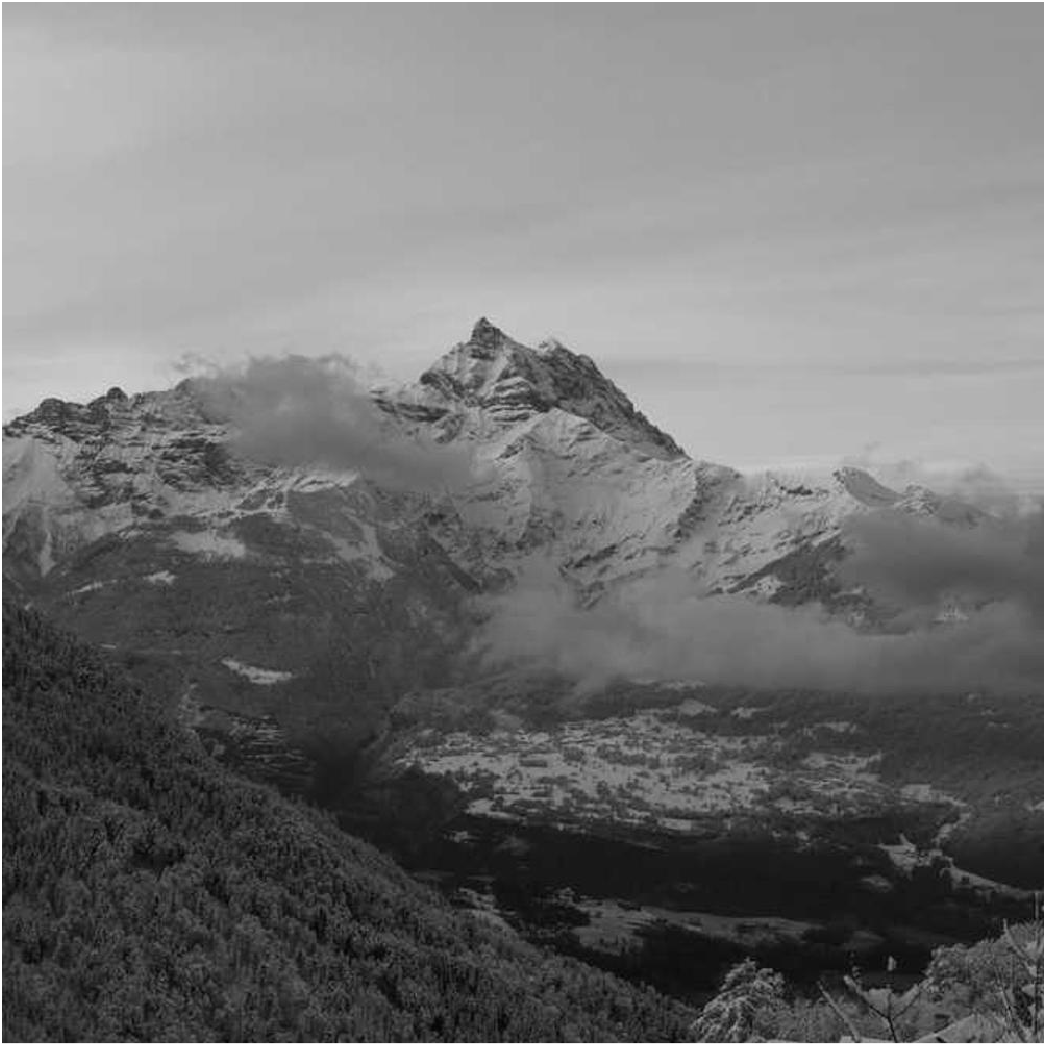
\includegraphics[width=\linewidth]{\mapa/slikaInput.png}
        \caption{Originalna slika.}
    \end{subfigure}
    \hfill
    \begin{subfigure}{0.49\linewidth}
        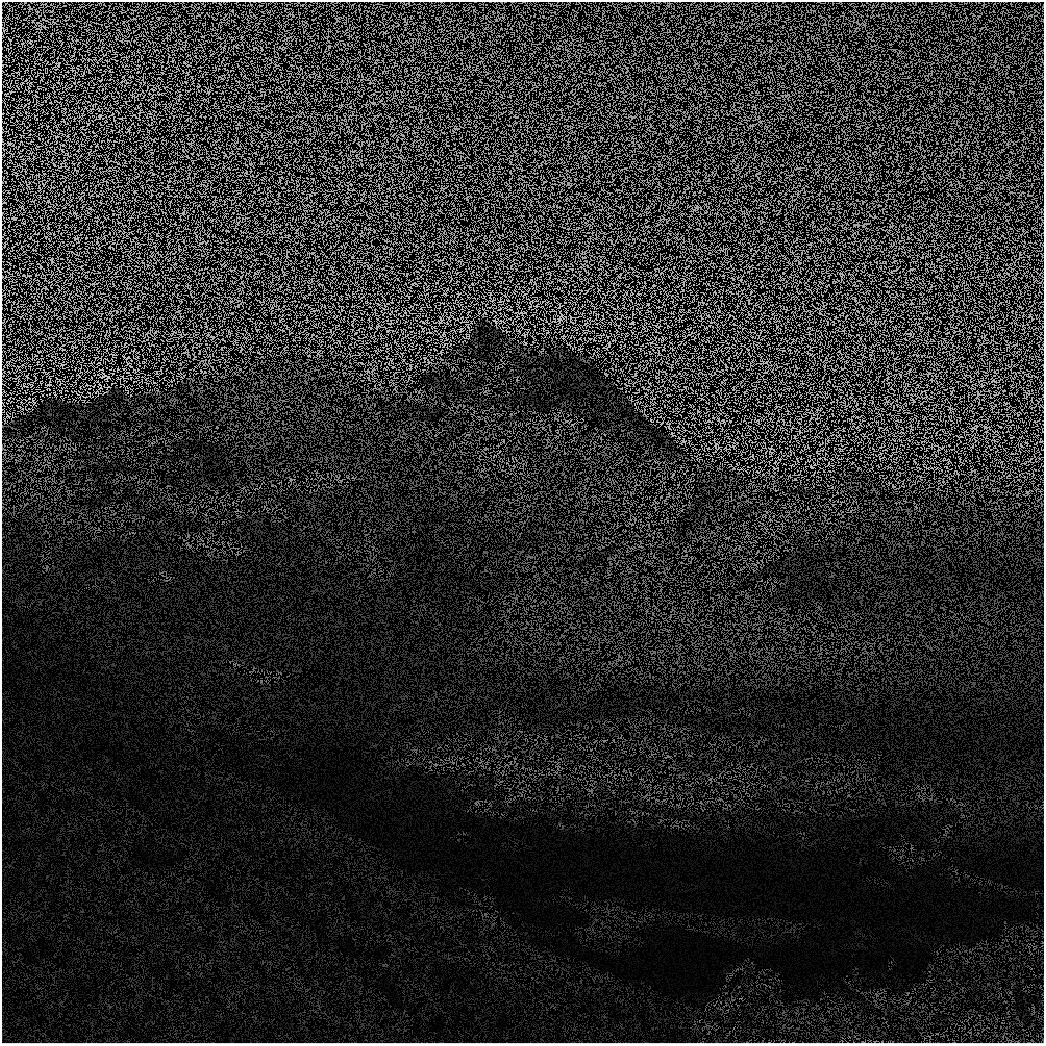
\includegraphics[width=\linewidth]{\mapa/slikaInput35.png}
        \caption{Slika s $35\%$ znanimi podatki.}
    \end{subfigure}
    \begin{subfigure}{0.49\linewidth}
        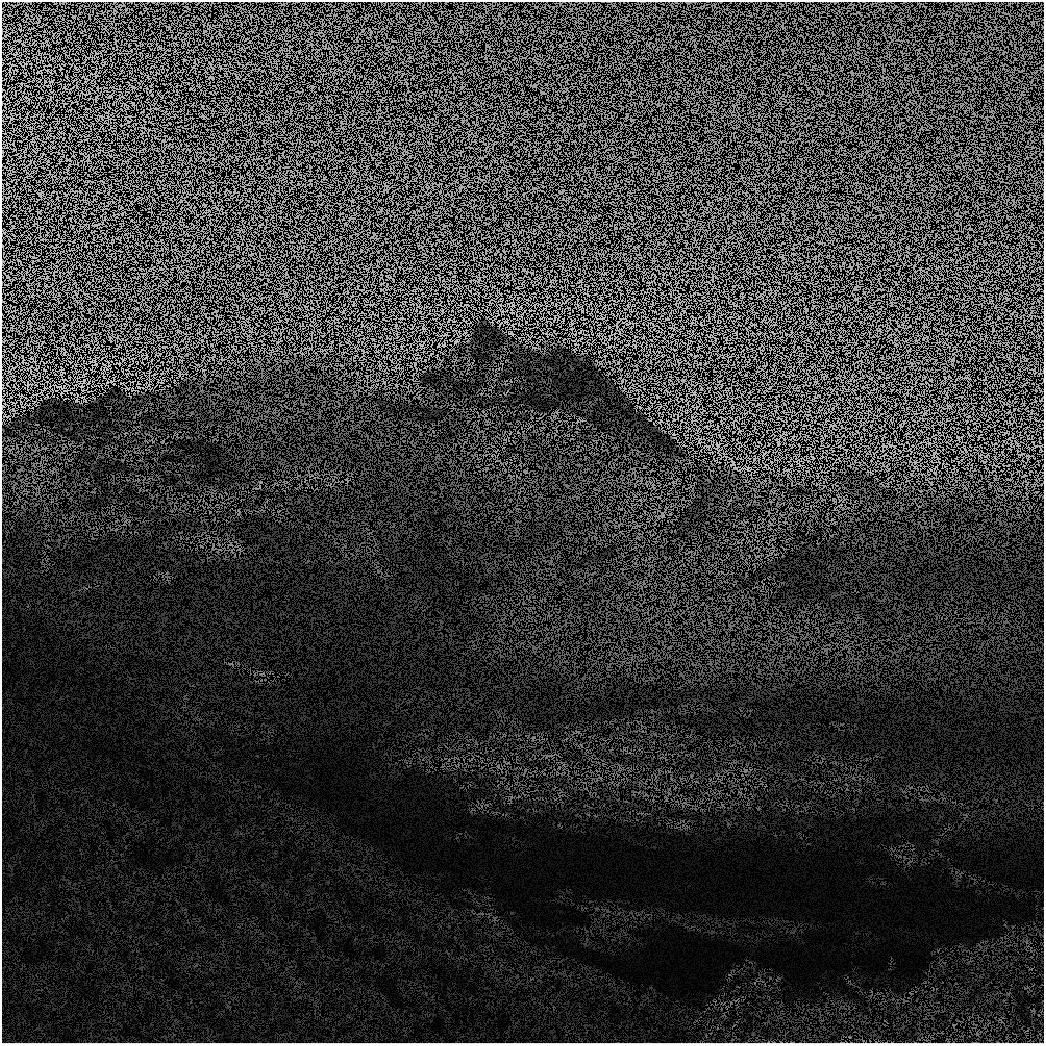
\includegraphics[width=\linewidth]{\mapa/slikaInput45.png}
        \caption{Slika s $45\%$ znanimi podatki.}
    \end{subfigure}
    \hfill
    \begin{subfigure}{0.49\linewidth}
        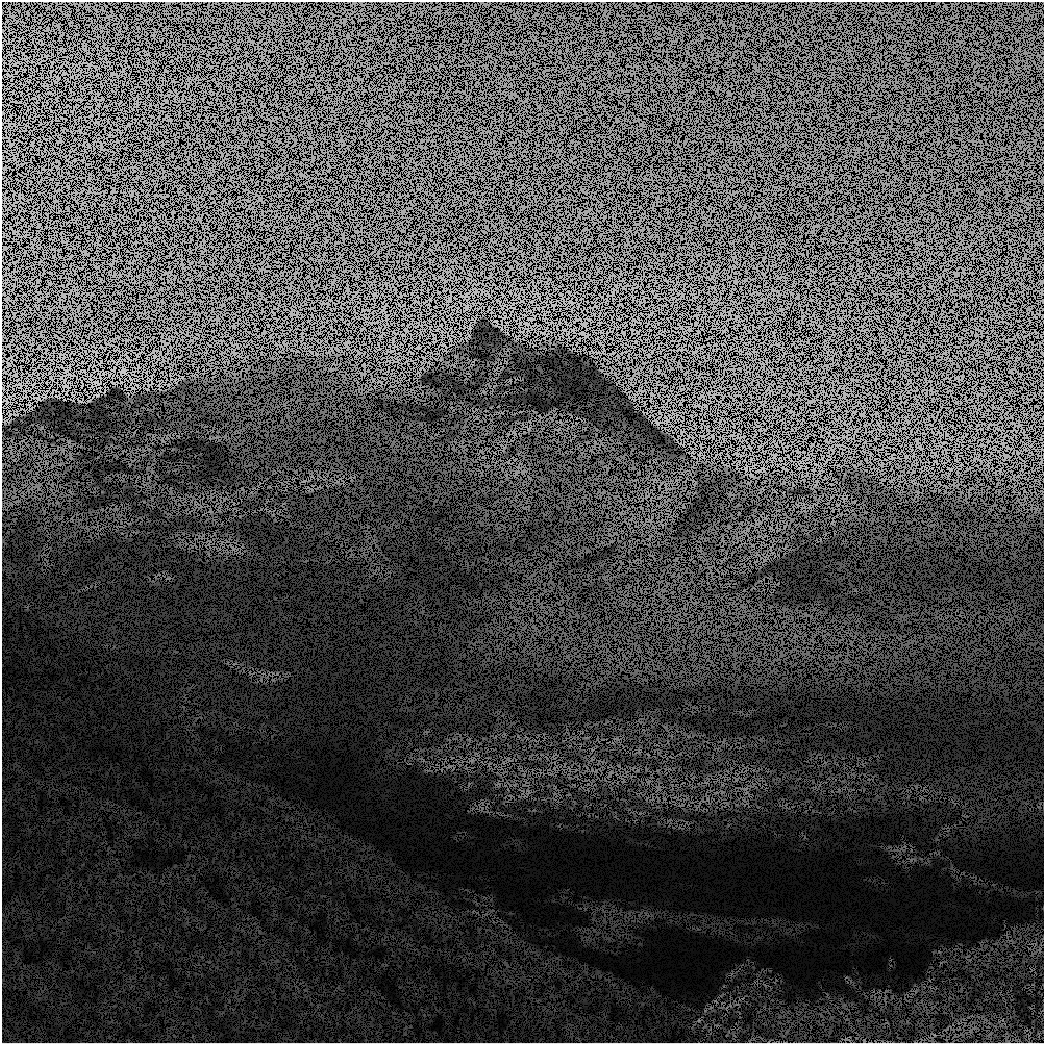
\includegraphics[width=\linewidth]{\mapa/slikaInput60.png}
        \caption{Slika s $60\%$ znanimi podatki.}
    \end{subfigure}
    \caption{Slika uporabljena za rekonstrukcijo. \cite{UnsplashGora}}
\end{figure}

\begin{figure}[!ht]
    \centering
    \begin{subfigure}{0.325\linewidth}
        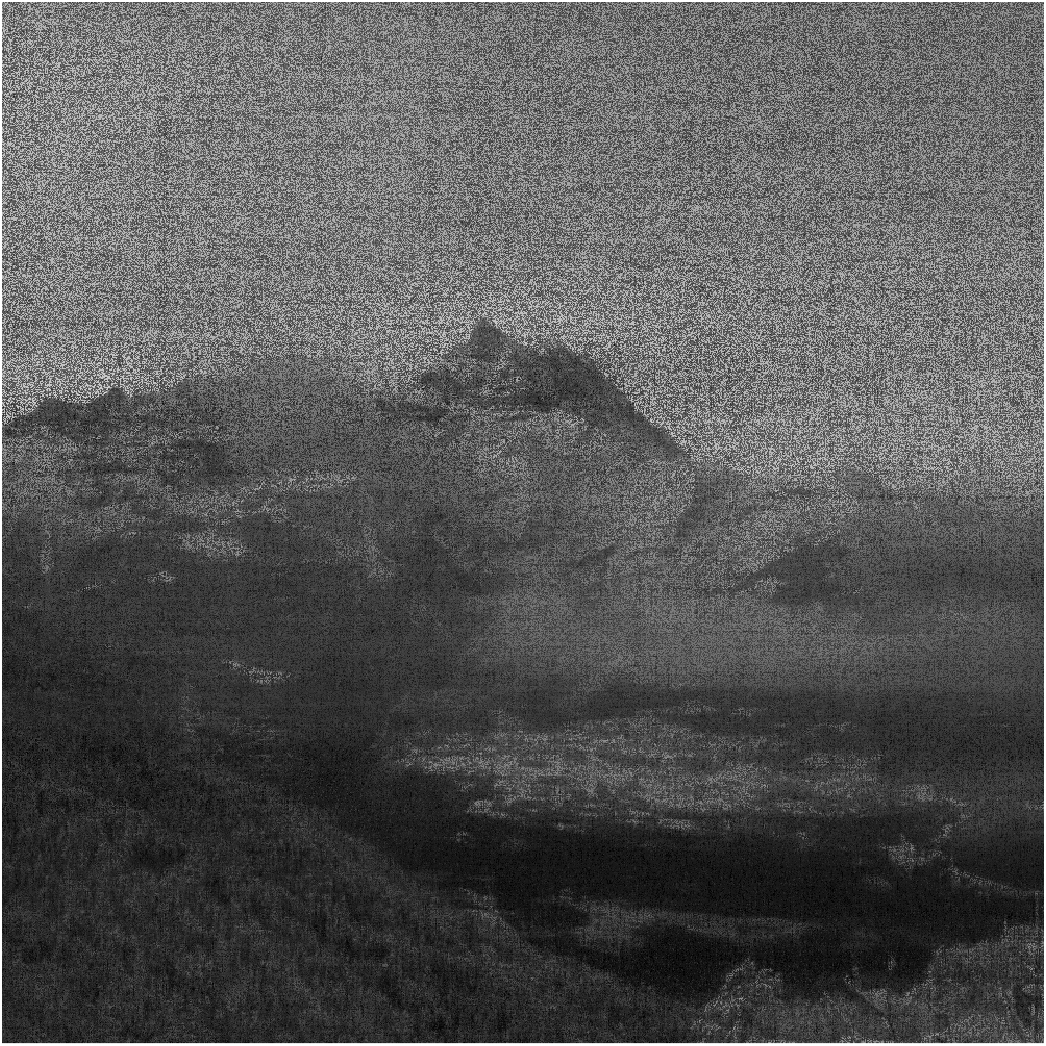
\includegraphics[width=\linewidth]{\mapa/slikaRez35SVT.png}
        \caption{SVT, $35\%$}
    \end{subfigure}
    \hfill
    \begin{subfigure}{0.325\linewidth}
        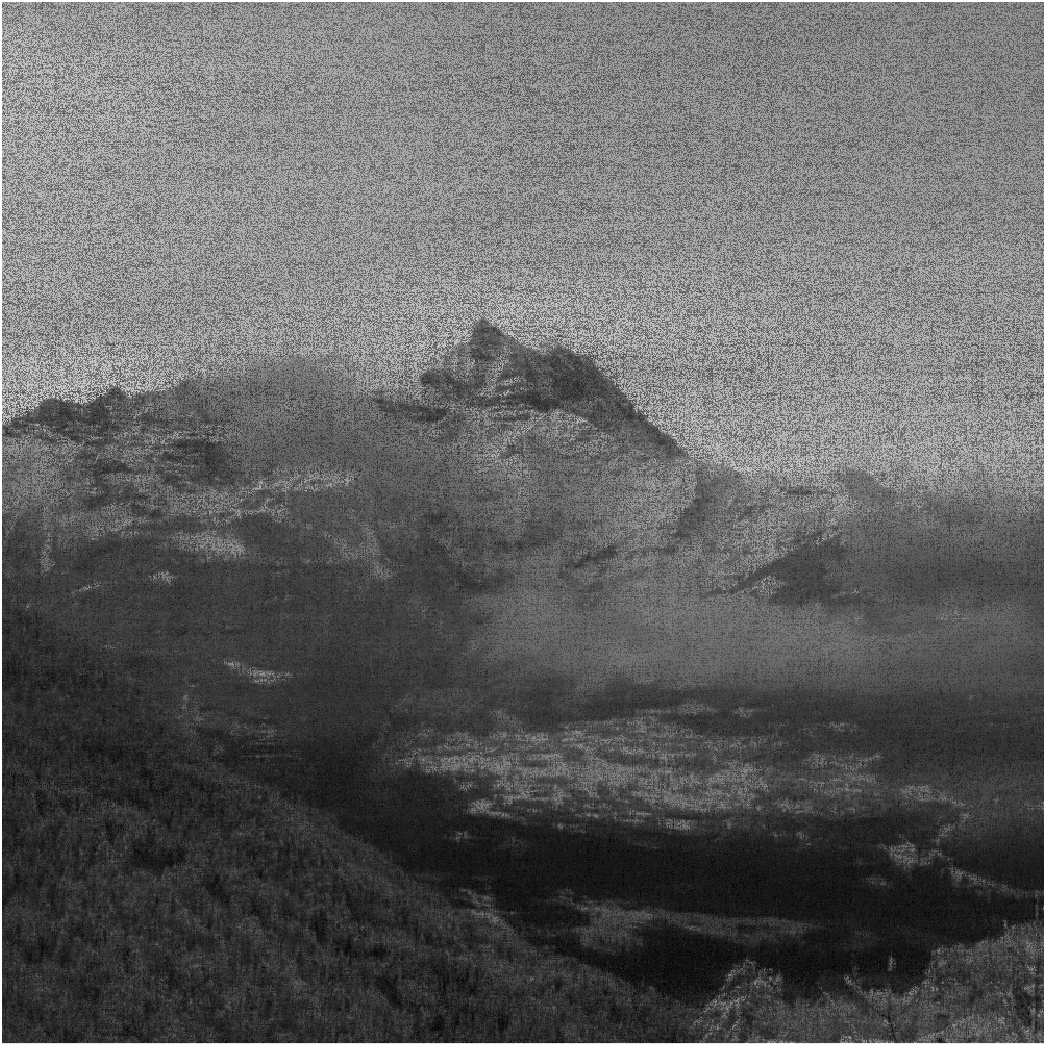
\includegraphics[width=\linewidth]{\mapa/slikaRez45SVT.png}
        \caption{SVT, $45\%$}
    \end{subfigure}
    \hfill
    \begin{subfigure}{0.325\linewidth}
        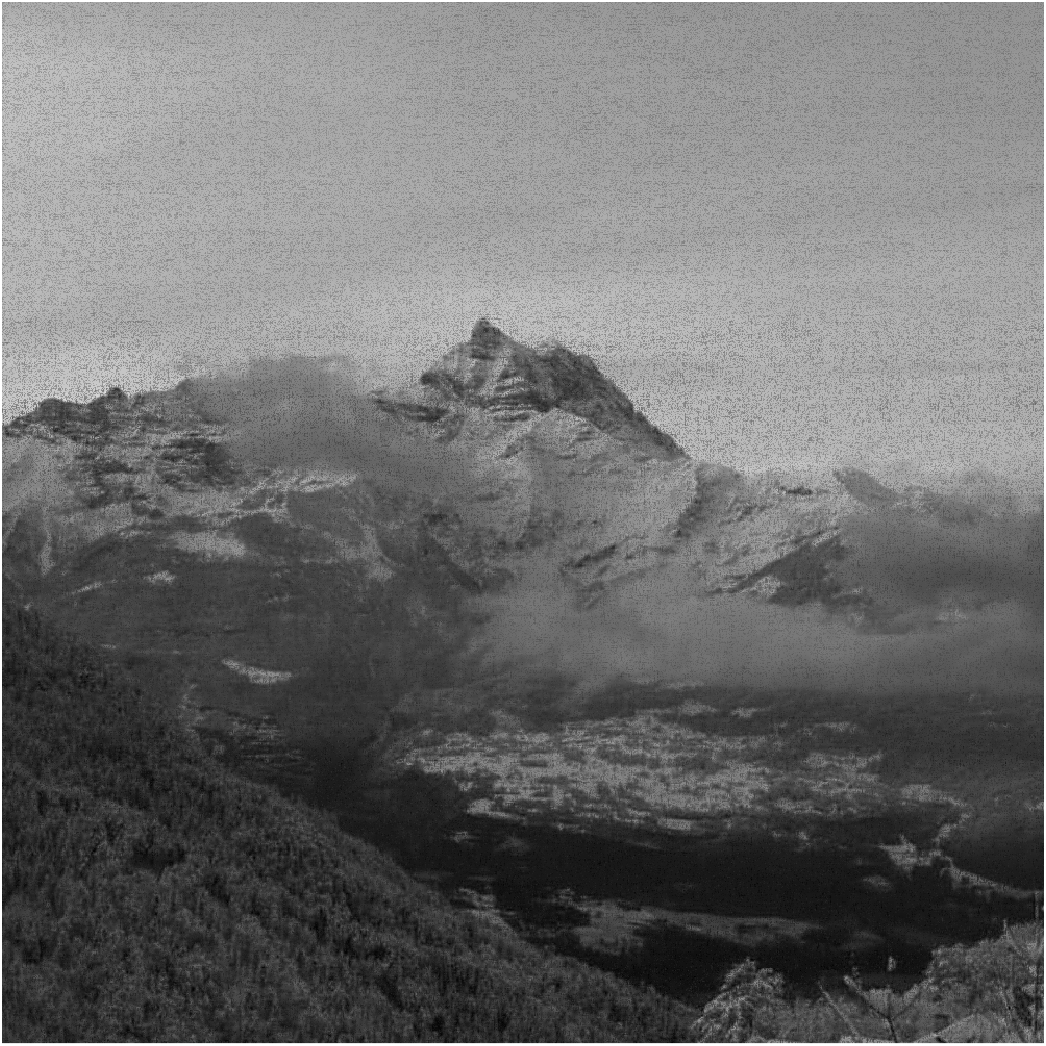
\includegraphics[width=\linewidth]{\mapa/slikaRez60SVT.png}
        \caption{SVT, $60\%$}
    \end{subfigure}
    \begin{subfigure}{0.325\linewidth}
        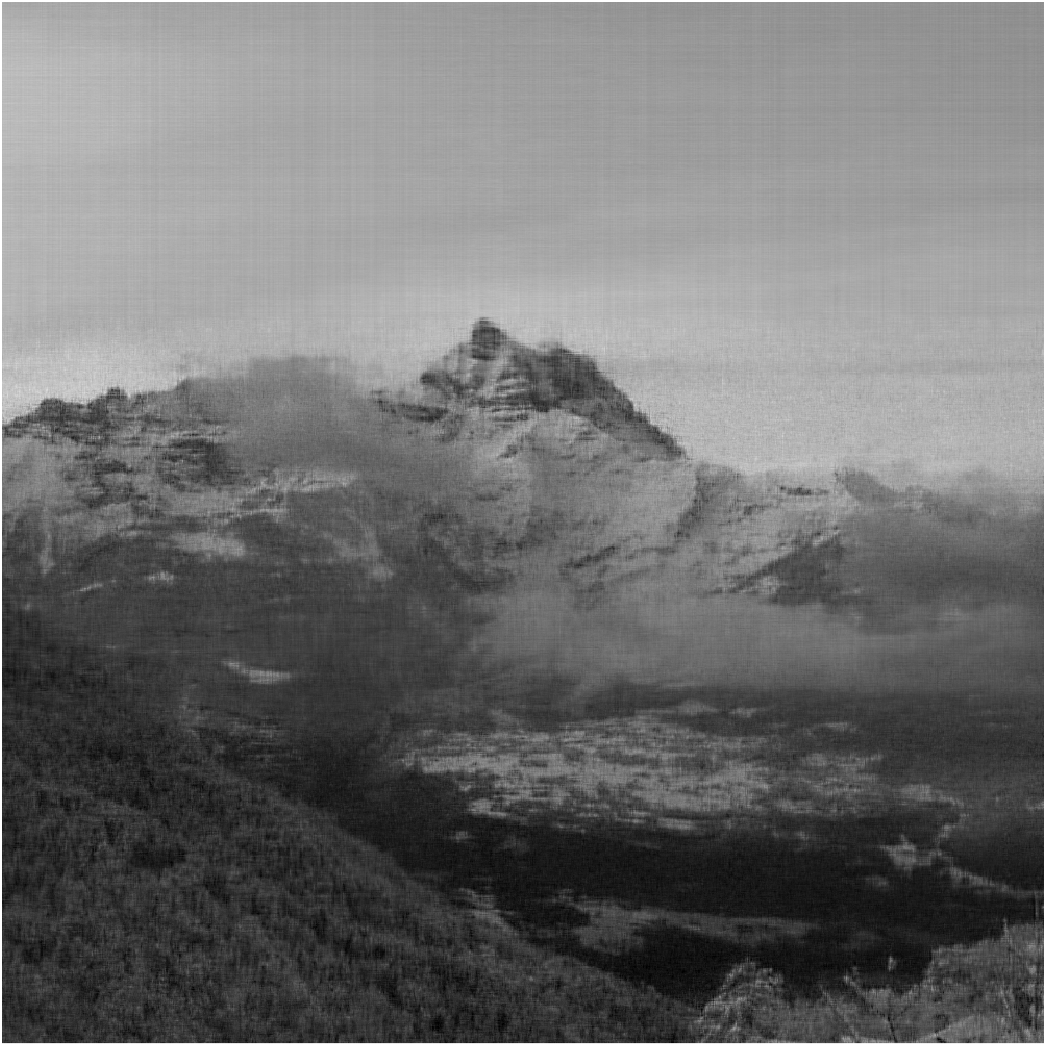
\includegraphics[width=\linewidth]{\mapa/slikaRez35TNNM.png}
        \caption{TNNM, $35\%$}
    \end{subfigure}
    \hfill
    \begin{subfigure}{0.325\linewidth}
        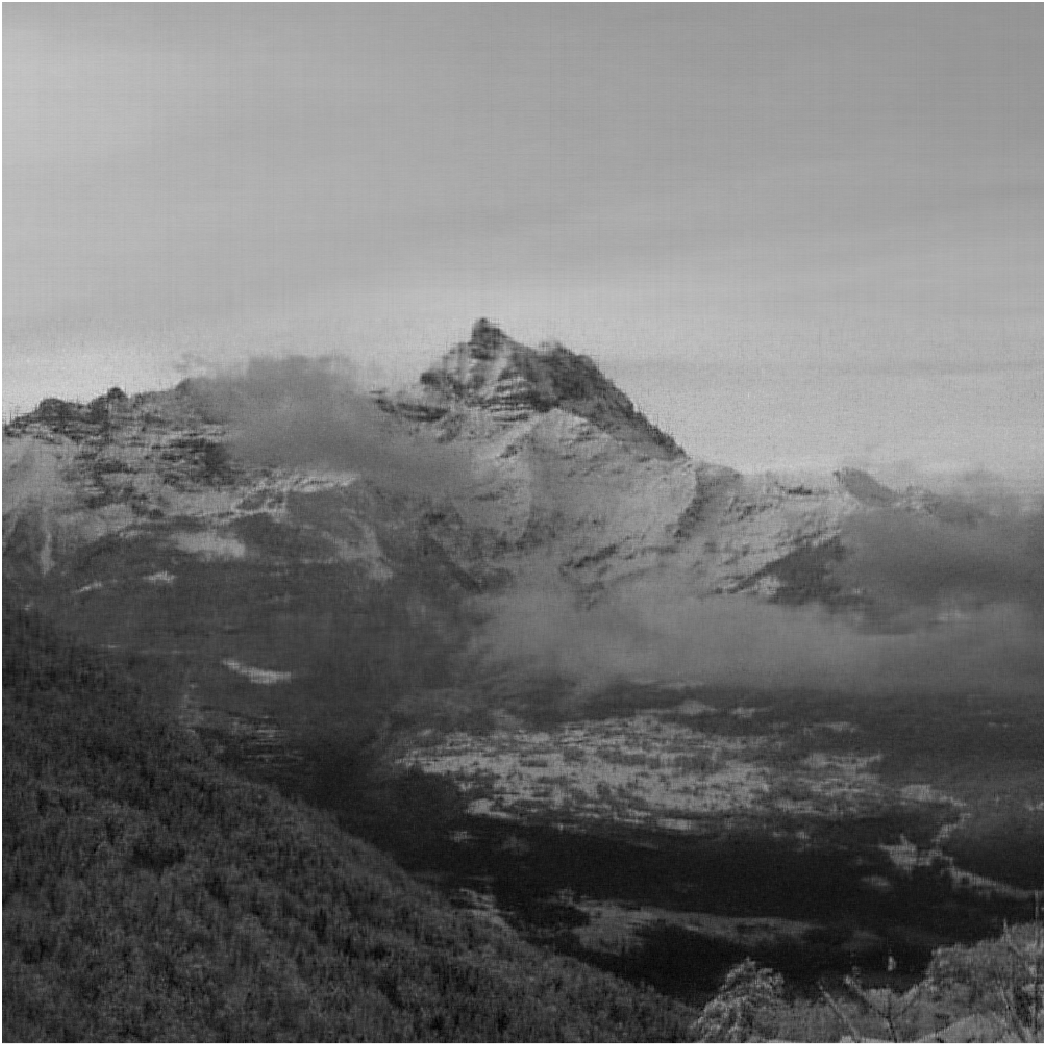
\includegraphics[width=\linewidth]{\mapa/slikaRez45TNNM.png}
        \caption{TNNM, $45\%$}
    \end{subfigure}
    \hfill
    \begin{subfigure}{0.325\linewidth}
        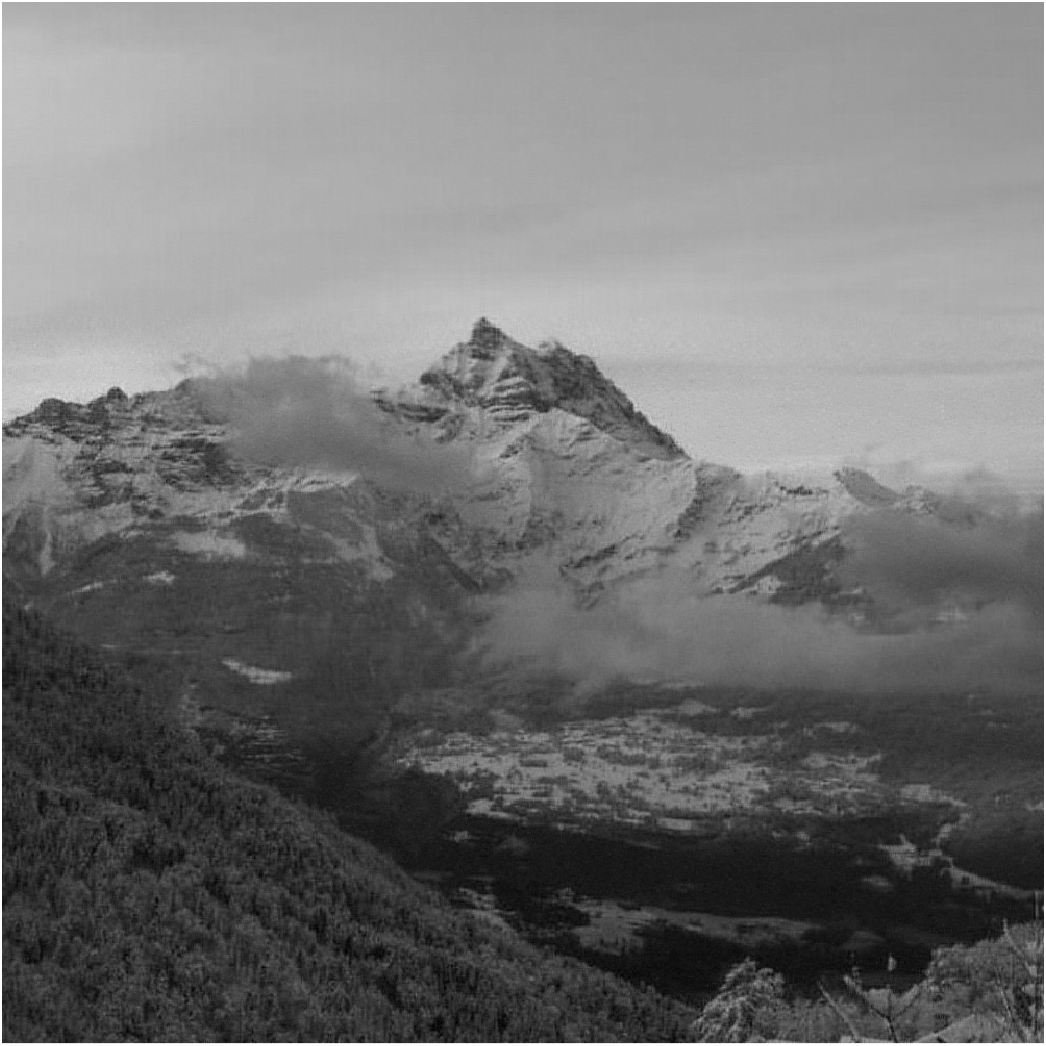
\includegraphics[width=\linewidth]{\mapa/slikaRez60TNNM.png}
        \caption{TNNM, $60\%$}
    \end{subfigure}
    \begin{subfigure}{0.325\linewidth}
        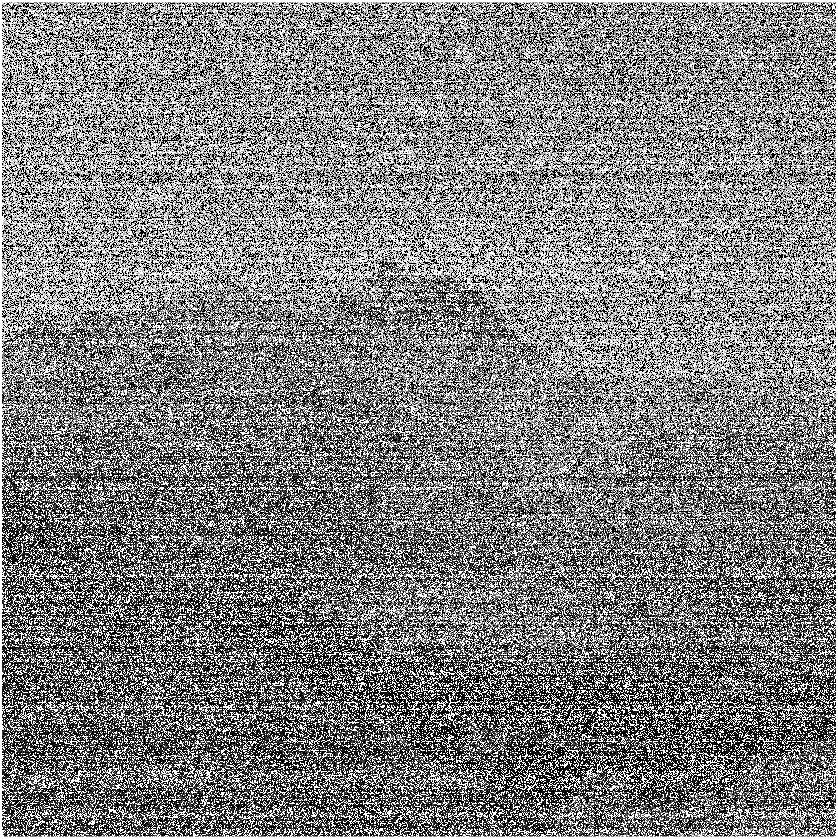
\includegraphics[width=\linewidth]{\mapa/slikaRez35ASD400.png}
        \caption{ASD, $35\%$}
    \end{subfigure}
    \hfill
    \begin{subfigure}{0.325\linewidth}
        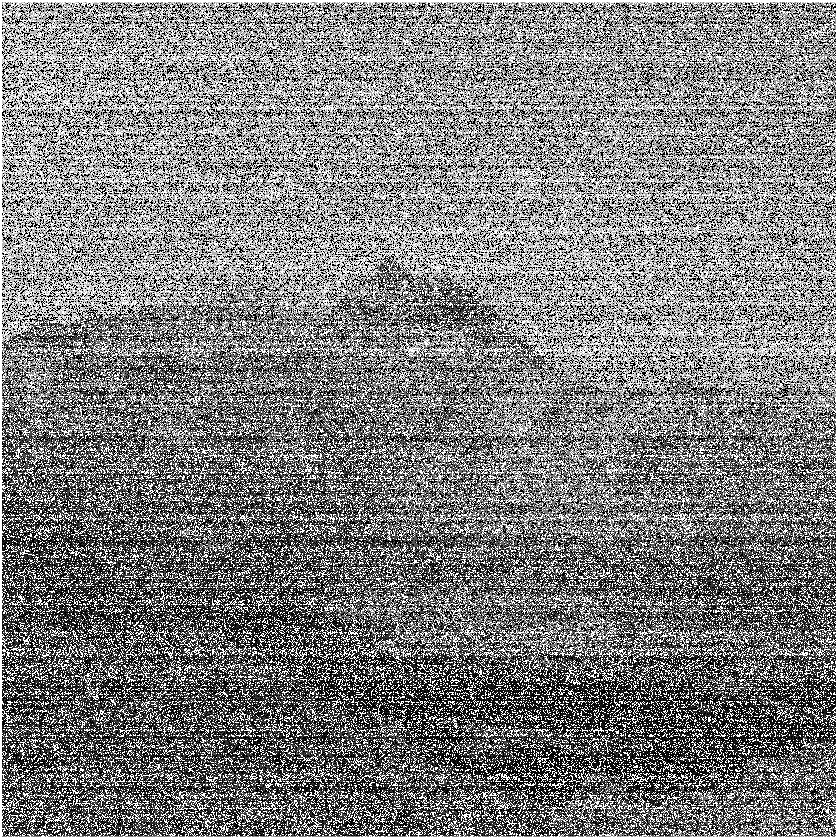
\includegraphics[width=\linewidth]{\mapa/slikaRez45ASD600.png}
        \caption{ASD, $45\%$}
    \end{subfigure}
    \begin{subfigure}{0.325\linewidth}
        %ASD 60?%
        \hfill
    \end{subfigure}
    \begin{subfigure}{0.325\linewidth}
        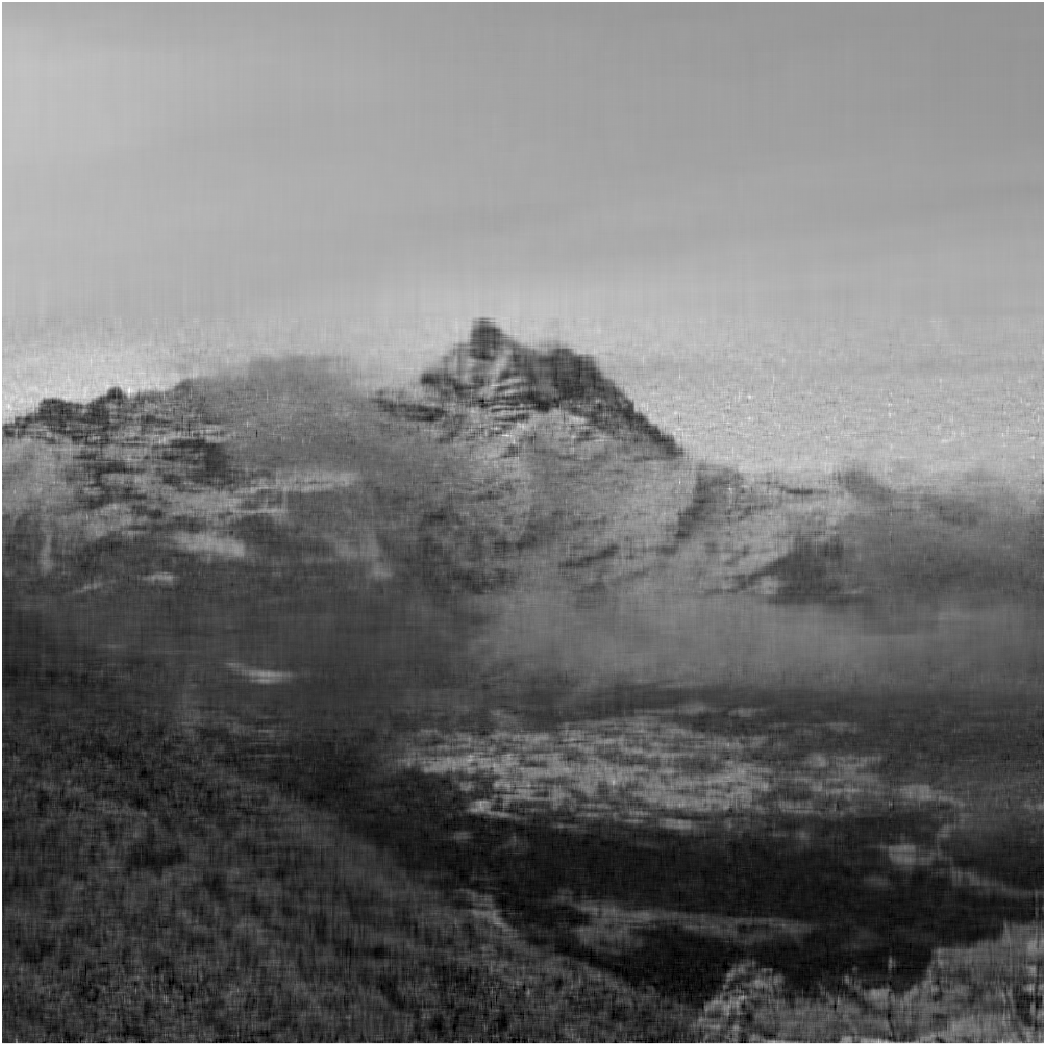
\includegraphics[width=\linewidth]{\mapa/slikaRez35LmaFIT50.png}
        \caption{LMaFit, $35\%$}
    \end{subfigure}
    \hfill
    \begin{subfigure}{0.325\linewidth}
        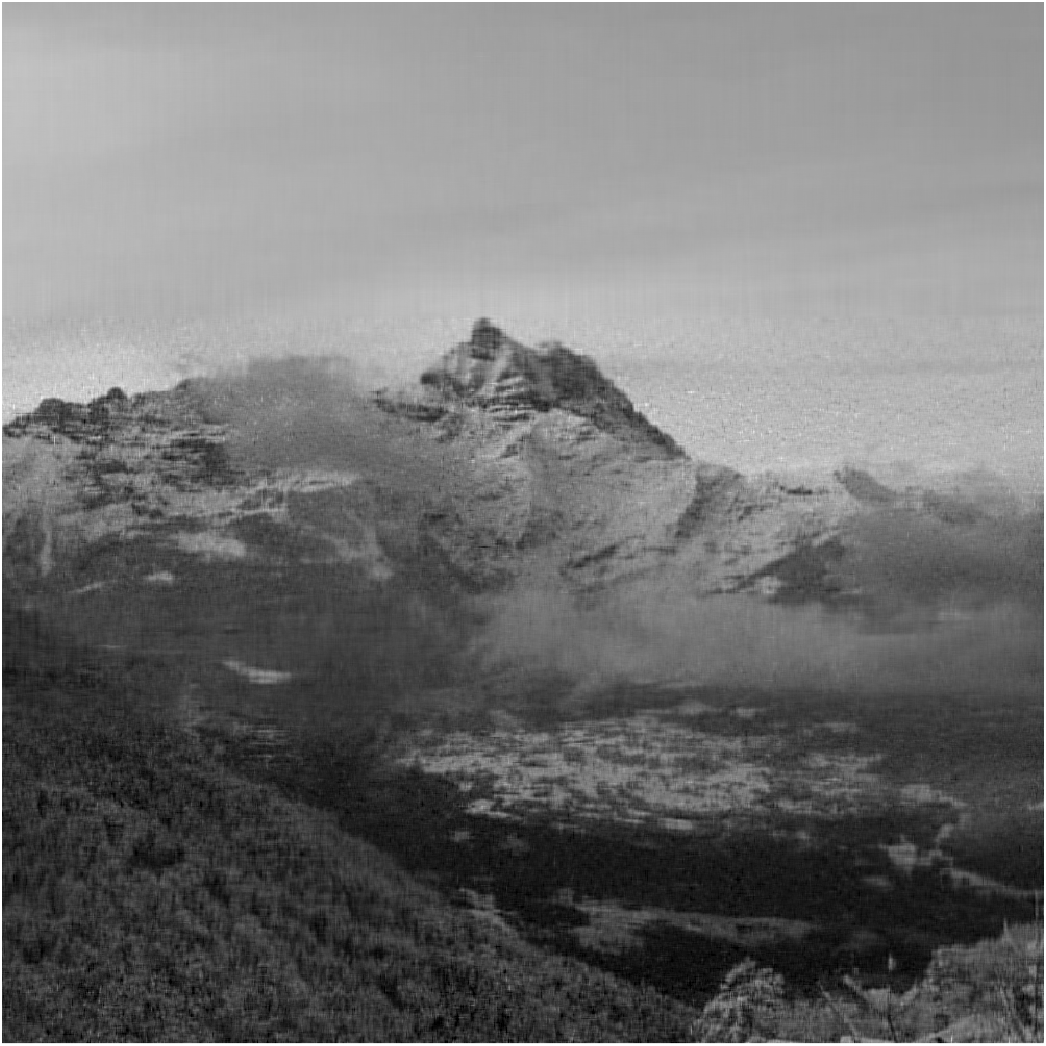
\includegraphics[width=\linewidth]{\mapa/slikaRez45LmaFIT73.png}
        \caption{LMaFit, $45\%$}
    \end{subfigure}
    \begin{subfigure}{0.325\linewidth}
        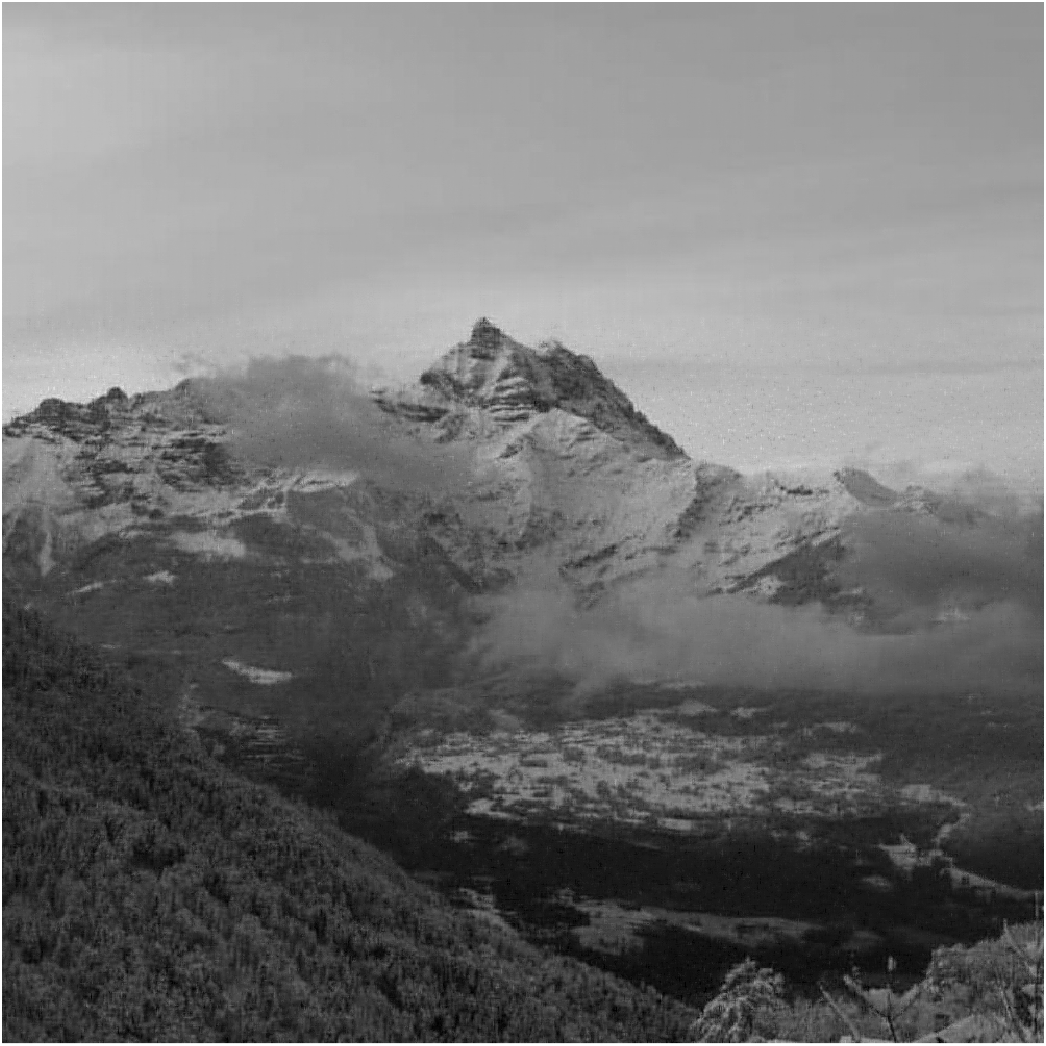
\includegraphics[width=\linewidth]{\mapa/slikaRez60LmaFIT77.png}
        \caption{LMaFit, $60\%$}
    \end{subfigure}
    \caption{Rekonstrukcija zašumljenih slik z uporabo različnih algoritmov in pri različnih odstotkih znanih vrednosti. Kratica pod sliko označuje uporabljen algoritem, odstotek za vejico pa odstotek znanih vrednosti.}
\end{figure}